%!TEX root = ../../../super_main.tex

\chapter{Issues and Solutions}

The launcher application seems to be working fine at a first glance, but at further inspection it has a lot of edge cases that cause it to crash when used for longer periods of time. In order to find these crashes we conducted a series of unstructured tests and UI/Application Exerciser Monkey (Monkey) \parencite{android_monkey} tests to explore the launcher and find bugs during the start of the first sprint. Monkey is a tool, which comes with the Android Debug Bridge (adb) \parencite{android_adb}, used to perform series of pseudo-random streams of user events to test the application UI under stress. We found the Monkey tool to be useful and it did help us find several issues in the code, e.g. concurrency issues when switching between tabs in the settings activity of the launcher.
\\\\
Android and general code mistakes might occur multiple times in code base, and will be corrected when discovered, but only the first discovered occurrence is mentioned in this chapter. 
\\\\
In addition to the issues discovered by using the Monkey tool, some requests from the costumers regarding design will also be described during this section.

%!TEX root = ../../../super_main.tex
\section{Crash in Settings Tab}
\label{sec:crash_in_settings_tab}

We have discovered a bug related to the settings menu in the launcher GUI during one of the initial automated monkey test of the GUI. The bug occurs when the different tabs of the settings menu are clicked in rapid succession, especially the tab where the user is able to select which android applications they want to see in the \giraf launcher.
\\\\
The cause of the bug is found to be a race condition caused by manipulation of a static reference called \androidinline{mAppInfoHashMap} on an \androidinline{AppViewCreationUtility} object. This manipulation happens from the main (GUI) thread and a background thread managed by a LoadApplicationTask. The reference was manipulated in two different methods \androidinline{updateAppInfoHashMap} and a method \androidinline{onClick} defined in an anonymous subclass of \androidinline{View.OnClickListener}. The race condition occurs because the \androidinline{onClick} is invoked on the GUI thread while the \androidinline{updateAppInfoHashMap} method is invoked on the a background thread, managed by a LoadApplicationTask, concurrently.   

\subsection{Solution}
\label{sub:crash_in_settings_tab_solution}
The race condition is resolved by using monitors, i.e. by utilizing the \androidinline{synchronized} Java keyword, in order to protect the critical sections where the \androidinline{mAppInfoHashMap} reference was manipulated. This ensures the only one task or thread has access to the variable at any time, and therefore the race condition can not happen.





%!TEX root = ../../../super_main.tex
\section{Fragment Manager}
\label{sec:fragment_manager}

When nesting Android \androidinline{Fragment} objects, i.e having a \androidinline{Fragment} which contains another \androidinline{Fragment} in its layout, it is imperative that the parent Fragments uses a \androidinline{FragmentManager} provided by a call to \androidinline{getChildFragmentManager} instead of the \androidinline{FragmentManager} provided by the parent activity. The \giraf-class \androidinline{AppManagementFragment} failed to do this.   

AppManagementFragment

%!TEX root = ../../../super_main.tex

\section{Fragment Constructors}
\label{sec:fragment_constructors}

According to the Android API documentation \parencite{android_dev_fragment} Android Fragment subclasses classes must make a public no-argument constructor, a default constructor, available. However the \giraf-class \androidinline{SettingsLauncher} failed to provide such a default constructor which caused crashes. The standard practice when sub classing \androidinline{Fragment} objects is to provide a static factory method, which creates a new instance of the \androidinline{Fragment} subclass, called \androidinline{newInstance}. \androidinline{newInstance} takes its arguments and passes them to the created \androidinline{Fragment} subclass object through an Android \androidinline{Bundle} instance.

%!TEX root = ../../../super_main.tex

\section{Inconsistent tab size in settings panel}

%!TEX root = ../../../super_main.tex

\section{Reengineering of Application Grid}
\label{sec:reengineering_of_application_grid}

When the launcher of the \giraf system is being used, and the user presses the drawer on the left-hand side, the application grid becomes smaller as a result of the drawer moving on the screen. The resulting smaller area has to be repopulated with icons, since the icons no longer have proper placements. Furthermore the application window currently has a fixed size, while the user is able to select as many applications as he/she wants. This means that if too many applications are chosen, they will surpass the size of the window, and therefore be pushed out of the window.
\todo[inline]{Add some figure that describes how the problem was solved}
The applications are currently being placed in the launcher by using LinearLayouts placed in rows, which then individually contain an amount of icons respective to the icon size. The computation of how many rows are needed, the location of all icons, etc., has a serious effect on performance and smoothness of the launcher. This gives the user a poor experience when interacting with the application, and we would therefore like to improve the launcher application such that it uses a ViewPager and a Grid structure instead. A ViewPager is the standard application showing method for phones and tablets, where the user is able to swipe from side to side between the different pages with applications on them. This is desirable since it gives the user a consistent experience with devices they usually use. A Grid is preferable over a rows of LinearLayouts since it is easier to build and populate with icons, which should result in increased performance. 
\\\\
There are furthermore issues with the applications being shown either several times or not at all upon loading the launcher. We assume this is caused by the way the LinearLayouts are being made and at which times the call to create a new view happens, and will therefore be resolved once the implementation is changed to a grid. 

\subsection{Solution}
\label{sub:reengineering_of_application_grid_solution}
\todo[inline]{Write how we solved the grid rework}



%!TEX root = ../../../super_main.tex
\section{Wrong User Permissions}
\label{sec:wrong_user_permissions}

In the \giraf-applications, there exists three different profile-types, namely \emph{Administrator}, \emph{Guardian}, and \emph{User}. Administrators have the widest permissions, and are allowed to create guardians and users. Guardians can administrate a subset of the users, for instance the users connected to a specific institution, or part of an institution. Users are allowed to use different applications, namely the ones that have been added to their profile by one of their guardians. 
\\\\
However, these different profile-types are not enforced correctly in the \launcher-application. Currently, guardian- and user profiles have access to the same features. For instance, a regular user may access the settings-panel and choose which applications that should be accessible for that particular user. This feature should only be available for guardians- and administrator profiles.
\\\\
Before a guardian hands the tablet to a user, the guardian needs to switch profile to that specific user, so that the system knows what features should be available. Only guardians should be allowed to switch profiles. Currently all profile types are able to switch profiles, meaning that regular users can switch to a guardian profile and thereby gain access to parts of the application that should otherwise be unavailable.

\subsection{Solutions}
\label{sub:wrong_user_permissions_solutions}

We fixed 

%!TEX root = ../../../super_main.tex
\section{Settings Alignment}
\label{sec:settings_alignment}

The settings tab in the launcher contains the different settings for the user. It was discovered during the development, that some of the settings in the panel were not aligned, which gave a bad user impression. We would like to change it so that all the settings in the settings panel are aligned to the left side, such that the panel has a consistent and smooth look. 

\todo[inline]{Insert picture here that shows the ugliness of the settings without the fix}

\subsection{Solution} 
\label{sub:settings_alignment_solution}
We discovered that the misplacement of the settings was caused by the way SwitchPreferences are made in Android. By default a SwitchPreference contains a picture to the left, then some text, and then a switch. As a result, the text is moved to the right to accommodate for the fact that a picture could be present. As we do not want to use pictures as an indicator for our SwitchPreference, we change the visibility of the hidden picture to be ``GONE'' instead. This makes the text able to use the space otherwise reserved for the picture, and the text is now nicely aligned with the settings below it. 




%!TEX root = ../../../super_main.tex
\section{Button Inconsistency}
\label{sub:button_inconsistency}

The graphical design of the GUI was found to be very inconsistent in general around in the \giraf-software suite. This issue was discovered by the \emph{SW606F15} group, who is the group responsible for user requirements and the graphical design guide of the project.
\\\\
In cooperation with this group it was found that the implementations of the GUI-components that existed needed refactoring based on the code quality and structure of the existing code base of GUI-components.
\\\\
One of the problems found by \emph{SW606F15} is illustrated in figure \figref{fig:button_inconsistency} where it can be seen that the settings button (top most button) and the logout button (lower most button) are very inconsistent in the graphical design. 

\begin{figure}[!htbp]
    \centering
    
\includegraphics[width=0.1\textwidth]{sprint_one/enforce_design_guide_in_settings/button_inconsistency}
    \caption{Example of inconsistent Buttons}
    \label{fig:button_inconsistency}
\end{figure}

This motivated \emph{SW606F15} to create a graphical design document which will be used to enforce a standard for the GUI \todo{Maybe insert the design document in the appendix and refer to it}. Furthermore, this design flaw was found in the GUI of the \launcher, which made us commit to the job of solving this problem. 
\\\\
To solve the button inconsistency, a standardized should be developed. This standard for buttons should correspond to the looks and feel described in the design document created by \emph{SW606F15}. 

\subsection{Solution}
\label{sub:solution}

At first, the design document indicated that the there should exist different button types. Each type should have a specific background color associated with it. For instance, buttons with user-actions should have a brown background as seen on \figref{fig:ugly_and_beautiful_buttons_example_one}. However, after implementing this feature, it was discovered that the users at \emph{Birken} did not like these new buttons, and would rather keep the look of the old buttons as seen on \figref{fig:ugly_and_beautiful_buttons_example_two}. However, consistency should still be enforced. This allows for consistent icons and background colors throughout the applications.\\

\begin{figure}[!htbp]
    \centering

    \begin{subfigure}[t]{0.3\textwidth}
    	\centering
        
\includegraphics[width=0.3\textwidth]{sprint_one/ugly_and_beautiful_buttons/button_redesign_beautiful}
        \caption{Colorful buttons}
        \label{fig:ugly_and_beautiful_buttons_example_one}
    \end{subfigure}
    \hspace{5em} 
    \begin{subfigure}[t]{0.3\textwidth}
    	\centering
        
\includegraphics[width=0.3\textwidth]{sprint_one/ugly_and_beautiful_buttons/button_redesign_ugly}
        \caption{Yellow buttons}
        \label{fig:ugly_and_beautiful_buttons_example_two}
    \end{subfigure}
    
    \caption{Solutions visualized}
    \label{fig:ugly_and_beautiful_buttons_example_solution}
\end{figure}

To create the standardized button a set of graphical icons were made by the \emph{SW606F15} group. These icons were then combined with a rounded square with a gradient background with the colors corresponding to the old buttons. All of this was made in the \mono{Giraf\_components}-module, which means that all applications are allowed to use this button. It is however still possible to use wrong icons, but we hope that the other groups will start to use this new button in their projects.
\\\\
Buttons are not the only thing that is inconsistent in the design, however we did not have enough time to create any other standardized components. 


%!TEX root = ../../../super_main.tex

\section{Unused Drawer}
\label{sec:unused_drawer}

During the development it was discovered by request of the users that the drawer of the sidebar in the \launcher was unused and not wanted anymore. In the initial version of this project the sidebar contained a drawer (open by the handle as seen in \figref{fig:button_inconsistency}). This problem was simply solved by removing the graphical indication of a drawer (see \figref{fig:ugly_and_beautiful_buttons_example_solution}) and removing the \androidinline{onClickListener} on the drawer. 

%!TEX root = ../../../super_main.tex

\section{Missing Apps in Application Grid}
\label{sec:missing_apps_racecondition}

We revealed an issue in the application grid, specifically with the background tasks that loads the applications and their icons. The application grid in the \launcher's Homeactivity would sometimes not show the applications. This issue occurs when the \launcher is to load its applications upon startup. The \launcher starts a background task in its onResume method which loads and prepares the applications to be shown.\\

This bug happens when the onResume method of the Homeactivity checks a boolean variable called \androidinline{mIsAppsContainerInitialized}, which was used in the previous solution to populating the application grid (see \secref{sec:reengineering_of_application_grid}). The previous solution included rebuilding a complicated layout called \androidinline{AppsContainer}, based on \androidinline{LinearLayout} objects, every time the grid had to change. This layout was built on a background thread in a \androidinline{LoadHomeActivityApplicationTask}. Once the layout was completed on the background thread, the variable mIsAppsContainerInitialized was set to true. A check on the variable was then performed to verify whether or not the application screen should be reloaded.

\begin{figure}[!htbp]
    \centering
    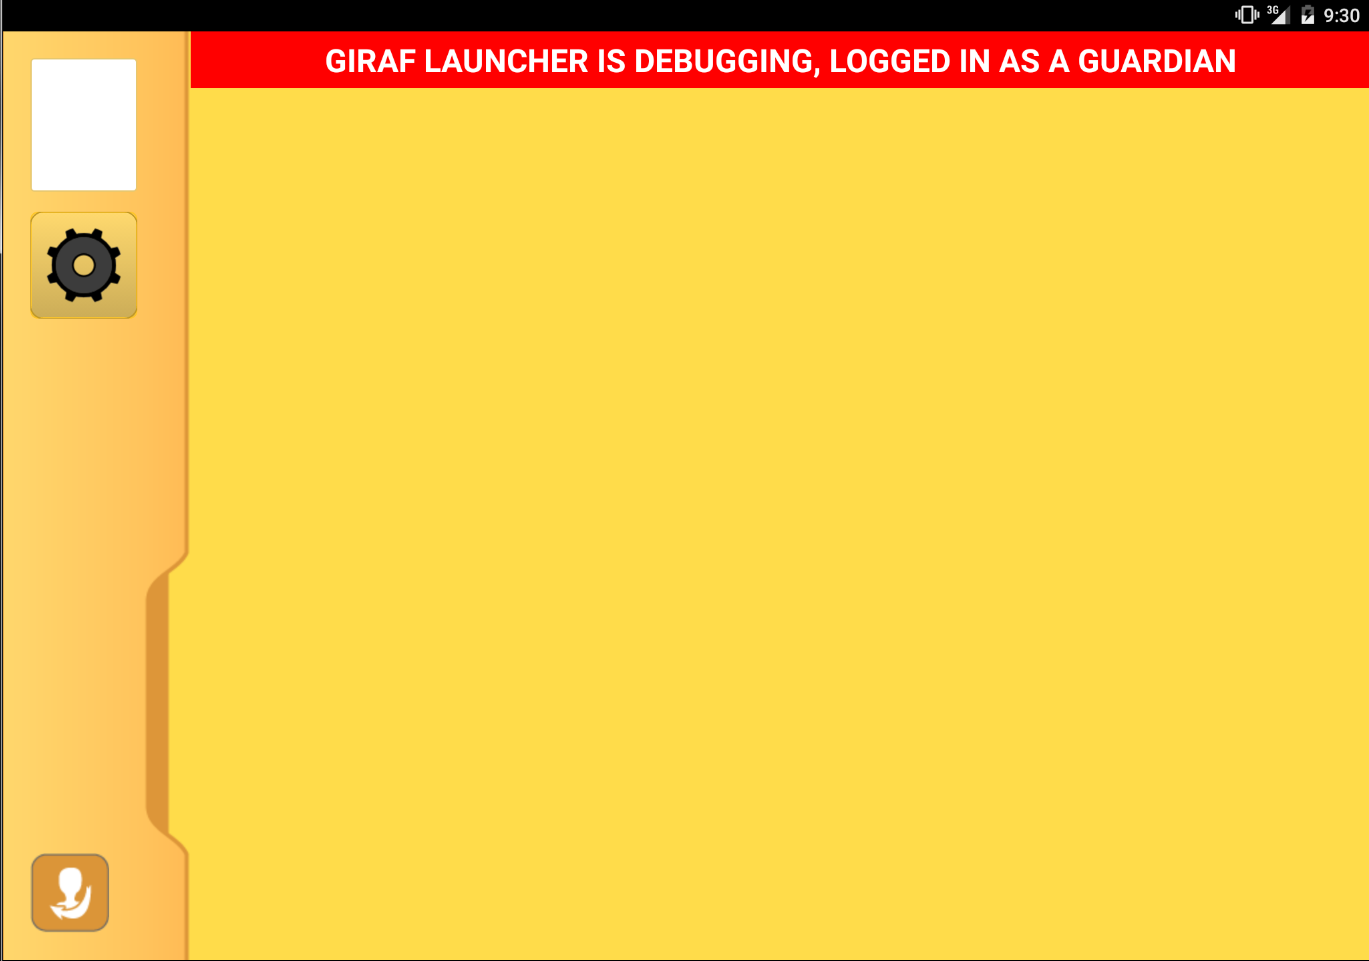
\includegraphics[width=\textwidth]{sprint_one/missing_app_icons/empty_app_icon_screen}
    \caption{Missing Apps}
    \label{fig:missing_apps}
\end{figure}

\subsection{Solution}
\label{sub:missing_apps_racecondition_solution}

The check on \androidinline{mIsAppsContainerInitialized} still happened after we implemented the changes described in \secref{sec:reengineering_of_application_grid}, as it did not seem to have any effect in most cases. Since it has been discovered that errors sometimes happen because of this check, and we no longer have any need to verify that we are done building any layouts, the piece of code has been removed. 

